\documentclass[conference]{IEEEtran}
\IEEEoverridecommandlockouts

\usepackage{cite}
\usepackage{amsmath,amssymb,amsfonts}
\usepackage{graphicx}
\usepackage{textcomp}
\usepackage{xcolor}
\usepackage{booktabs}
\usepackage{multirow}
\usepackage{url}
\usepackage[ruled,vlined]{algorithm2e}
\usepackage{amsthm}
\newtheorem{proposition}{Proposition}
\newtheorem{corollary}{Corollary}[proposition]
\theoremstyle{remark}
\newtheorem{remark}{Remark}
\newcommand{\TBD}{\textit{pending}}

\def\BibTeX{{\rm B\kern-.05em{\sc i\kern-.025em b}\kern-.08em
    T\kern-.1667em\lower.7ex\hbox{E}\kern-.125emX}}

\begin{document}

\title{FairPoC: Convergence-Stable Proof of Contribution for\\
Auditable Federated Learning via ERC-20 Smart Contracts}

% ICBC 2027 IS DOUBLE-BLIND. Identifying author block kept below as
% comments; restore it for the camera-ready version.
%\author{\IEEEauthorblockN{Derara Senay Shanka and Peter Shaojui Wang}
%\IEEEauthorblockA{Department of Computer Science and Information Engineering\\
%National Taiwan University of Science and Technology, Taipei 106, Taiwan\\
%E-mail: derjan06@gmail.com; shaojuiwang@mail.ntust.edu.tw\\
%Corresponding author: Peter Shaojui Wang}}
\author{\IEEEauthorblockN{Anonymous Submission}
\IEEEauthorblockA{Paper ID: \textit{(assigned at submission)}}}

\maketitle

\begin{abstract}
Federated learning requires a mechanism to reward participants in
proportion to their data contribution, but Shapley-based and
leave-one-out metrics degrade once the global model converges, and
existing systems distribute rewards through a central server with no
public audit trail. We propose \textbf{FairPoC}, which scores
contributions using normalised gradient norm --- stable throughout
training --- and settles rewards through ERC-20 smart contracts with
stake-and-slash enforcement: clients whose Proof-of-Contribution score
falls below 30\% of equal share are automatically slashed and
blacklisted, with no trusted intermediary required for settlement.
Across four non-IID regimes on CIFAR-10 and FashionMNIST, FairPoC
achieves the highest accuracy in all 8 configurations and the highest
GT-Fairness in 4 of 8, with consistent gains over all baselines across
the three moderate non-IID regimes on CIFAR-10. Under adversarial evaluation, free-rider
attacks incur a net loss of $1.67\times$ the staked amount and
gradient-inflation is capped below equal share by median-clip
normalisation. Settlement costs under \$0.12 per round for 10 clients
and requires no custom consensus, deploying on any EVM-compatible chain.
\end{abstract}

\begin{IEEEkeywords}
federated learning, blockchain, proof of contribution, non-IID, ERC-20,
smart contracts, stake-and-slash, adversarial robustness, fairness, gradient norm
\end{IEEEkeywords}

%----------------------------------------------------------------------
\section{Introduction}

Federated learning (FL)~\cite{mcmahan2017communication} allows multiple
clients to train a shared model on their local data, with only model
updates communicated to a central aggregator. This paradigm is
attractive for privacy-sensitive domains such as healthcare, finance,
and IoT~\cite{nguyen2021federated}. However, FL introduces a fundamental
economic problem: clients contribute heterogeneous amounts of value, yet
standard aggregation schemes reward all participants uniformly. Under
non-IID data distributions -- where clients hold skewed, non-representative
class subsets -- uniform reward policy over-rewards low-contribution
clients and under-rewards those with rare, high-value
data~\cite{zhan2021incentive, zhao2018federated}.

The consequences are practical. A rational client that observes its
scarce data is rewarded identically to a low-quality contributor will
reduce participation or withdraw, degrading the
federation~\cite{song2019profit}. Incentive mechanisms for FL have been
studied~\cite{wang2020measure, gradient_driven_fairness2021}, but
predominantly rely on a central server to distribute rewards with no
externally verifiable record -- participants must trust the server's
claimed allocation, which is unauditable in cross-organisational
deployments.

Blockchain technology offers \emph{auditable} enforcement: once a reward
distribution rule is encoded in a smart contract, execution is publicly
verifiable and tamper-evident~\cite{buterin2014ethereum}.
Behera et al.~\cite{behera2021federated} show that Ethereum smart
contracts can encode FL incentivization rules based on a scalar
contribution derived from weight updates. BLADE-FL~\cite{bladefl2022}
integrates blockchain consensus into a decentralised FL aggregation
framework. PoShapley-BCFL~\cite{poshapley2023} encodes Shapley-based
contribution into blockchain consensus. However, these works share a
common limitation: Shapley values and leave-one-out (LOO) contributions
collapse toward zero as the global model converges, making contribution
measurement unreliable in late training stages~\cite{poshapley2023}.
Furthermore, existing scalar contribution
metrics~\cite{behera2021federated} are based solely on weight-update
magnitude and do not account for distributional diversity -- a key
dimension of value under non-IID conditions.

Recent work proposes multidimensional contribution scores combining
reputation, data size, gradient diversity (Jensen-Shannon divergence),
and model performance, demonstrating improved fairness on heterogeneous
FL tasks~\cite{wang2020measure, gradient_driven_fairness2021}.
However, such approaches do not integrate with blockchain for
tamper-evident enforcement and do not address convergence-stability of
diversity signals.

We address these gaps with \textbf{FairPoC}:
\begin{enumerate}
  \item \textbf{A contribution signal that stays discriminative at
        convergence.} We score clients by normalised gradient norm, a
        heterogeneity-driven quantity that does not vanish once the
        global model saturates. Marginal-utility metrics (Shapley,
        leave-one-out) lose the ability to separate clients at
        precisely the point where reward allocation must still be
        enforced.
  \item \textbf{A non-circular protocol for evaluating contribution
        fairness.} GT-Fairness measures alignment between
        \emph{ground-truth} data quality and reward, rather than
        between reward and the system's own score. It is therefore
        distinct from dispersion measures such as the Gini coefficient
        of payouts~\cite{he2026blockflmd2c}, which are minimised by
        paying every client equally regardless of contribution.
  \item \textbf{Gradient-magnitude scoring is a manipulable primitive,
        and median-clip normalisation corrects it.} We characterise the
        self-amplifying failure mode of max-norm scoring under gradient
        inflation and show that median-clip removes the attacker's
        advantage, driving net gain below $1\times$.
  \item \textbf{Practical on-chain enforcement.} Stake-and-slash
        through standard ERC-20 interfaces, requiring no custom
        consensus, with measured gas costs. We claim deployment
        practicality here rather than novelty: on-chain reward
        enforcement is already established~\cite{rashid2025tffl,
        dong2022flock}.
\end{enumerate}

%----------------------------------------------------------------------
\section{Related Work}

\subsection{Contribution Measurement in FL}

Shapley-value approximation~\cite{shapley1953value, song2019profit,
wang2020measure} is the standard for FL contribution scoring but has two
practical problems: $O(2^n)$ exact computational complexity and
convergence instability (marginal contributions collapse as the model
saturates).
Xu et al.~\cite{gradient_driven_fairness2021} propose gradient-driven
reward allocation: each client is rewarded proportionally to the inner
product of its gradient with the collaborative model's final gradient,
guaranteeing equitable distribution by construction.
Their approach targets centralised collaborative ML with no blockchain
component and relies on gradient direction rather than scale.
FairPoC uses normalised gradient \emph{norm} (scale), a simpler
closed-form signal that is independent of the consensus gradient
direction and therefore stable throughout training, whereas
inner-product-based methods converge toward the mean gradient and
can lose client differentiation at convergence.
Unlike these approaches, which assume a trusted central coordinator for
distribution, FairPoC encodes rewards in an ERC-20 contract, enabling
auditable, tamper-evident distribution with no custom consensus.

\subsection{Blockchain-Assisted FL}

Kim et al.~\cite{kim2019blockchained} first proposed recording FL model
updates on blockchain for auditability. BLADE-FL~\cite{bladefl2022}
replaces the central aggregator with a blockchain-based consensus
mechanism where clients compete to generate blocks containing verified
model updates. PoCL~\cite{pocl2024} proposes a multi-winner blockchain
consensus algorithm that redistributes proof-of-work computation toward
FL training. PoShapley-BCFL~\cite{poshapley2023} encodes Shapley-based
contribution scores into a custom blockchain consensus. Behera et
al.~\cite{behera2021federated} use Ethereum smart contracts with a
scalar contribution metric derived from weight-update magnitude.

FLock~\cite{dong2022flock, dong2024flock} proposes on-chain
stake-and-slash for FL defence via smart contracts, where validators
forfeit deposits for submitting poisoned updates.
FairPoC shares the enforcement philosophy but differs in purpose:
FLock targets Byzantine poisoning defence with peer-to-peer model
evaluation; FairPoC targets \emph{contribution-proportional reward
fairness} under non-IID data, pairing slash with a non-IID-aware
PoC score and a non-circular GT-Fairness evaluation protocol.
Relative to this line of work, FairPoC replaces Shapley values and
weight-update scalars with a normalised gradient norm that remains
discriminative at convergence, and deploys through standard ERC-20
interfaces rather than a custom consensus rule. Earlier schemes that
place contribution evaluation on chain do so chiefly to remove reliance
on a semi-trusted scoring server~\cite{huang2024bcontrib}, which is a
different objective from the one pursued here.

\subsection{Reputation-Based Trust and Incentives in Blockchain FL}

A parallel line of work scores clients by \emph{trustworthiness} rather
than by contribution. TFFL~\cite{rashid2025tffl} builds a hybrid
subjective-logic reputation from time-decayed counts of positive and
negative interactions, weights it by data quality (Earth Mover's
Distance), performance and reliability, and distributes rewards through
six Solidity contracts using cooperative game theory with Nash, Pareto
and core guarantees. TAFL~\cite{rashid2026tafl} extends the same
reputation machinery into a detection, probationary-isolation and
gated-reintegration lifecycle, committing reward tuples to an auditable
ledger. Both are non-IID aware and both enforce rewards on chain.
FairPoC therefore does not claim novelty from that combination.

The distinction lies in what the score measures. Reputation in TFFL
accumulates from whether an update was \emph{flagged} by an attack
detector, which answers whether a client is trustworthy.
Contribution-proportional reward requires a different quantity, namely
how much each client added. TFFL allocates that share by Shapley value,
and this is where the signal fails. Marginal-contribution scores are
driven by the improvement a client makes to global accuracy, and that
improvement vanishes for every client simultaneously as the model
saturates, so the scores lose their ability to discriminate exactly when
the model is most valuable. The degeneracy is already acknowledged in the
Shapley literature, though not named as such: GTG-Shapley~\cite{gtgshapley2022}
discards any round whose total marginal gain falls below a threshold and
returns \emph{zero} for every participant in it, and Geimer et
al.~\cite{geimer2025volatility} report that Shapley-based allocations are
unstable across aggregation rules. Figure~\ref{fig:stability} quantifies
the same effect over training time: by round 30 of 50 the leave-one-out
signal has collapsed to near zero for every client, while the normalised
gradient norm remains discriminative throughout.

FairPoC's contribution is thus not the pairing of non-IID-aware scoring
with on-chain enforcement, which TFFL already provides, but a contribution
signal that remains non-degenerate at the point where reward allocation
and slashing must still be enforceable.

%----------------------------------------------------------------------
\section{System Design}

\subsection{Architecture Overview}

FairPoC has three roles: \emph{clients}, an \emph{aggregator}, and the
\emph{FairPoC smart contract}. Algorithm~\ref{alg:fairpoc} summarises
the per-round protocol.

\begin{algorithm}[t]
\caption{FairPoC Training Protocol}
\label{alg:fairpoc}
\KwIn{Global model $\theta^{(0)}$, rounds $T$, clients $\{1\ldots n\}$}
\For{$t = 1$ \KwTo $T$}{
  Aggregator broadcasts $\theta^{(t)}$ to all clients\;
  Each client $i$ trains locally, produces $\Delta w_i$\;
  Clients send $\Delta w_i$ to aggregator\;
  Aggregator computes PoC scores $s_i$ (Eq.~\ref{eq:poc})\;
  Aggregator calls \texttt{submitAndSettle($s_i$)} on-chain\;
  Contract mints and transfers tokens $\propto s_i$\;
  $\theta^{(t+1)} \leftarrow \sum_i \frac{s_i}{\sum_j s_j} \theta_i^{(t)}$\;
}
\end{algorithm}

The aggregator computes contribution scores and writes them to the
contract via \texttt{submitAndSettle()}. The smart contract then executes reward
distribution deterministically and immutably: once scores are posted,
no party -- including the aggregator -- can alter the resulting token
transfer. This makes the distribution step \emph{auditable and
tamper-evident}: any participant can verify every reward on-chain. Note
that score computation itself remains at the aggregator; full
trustlessness of scoring would require on-chain gradient verification,
which we identify as future work.

\subsection{Smart Contract Design}

\texttt{FairPoC.sol} extends ERC-20~\cite{erc20} with three on-chain
functions encoding both reward distribution and adversarial defence.
\texttt{stake()} locks a per-round deposit before training begins.
\texttt{submitAndSettle()} is called once per round by the aggregator:
for each client it atomically checks whether the PoC score exceeds
$30\%$ of equal share (a threshold that tolerates mild underperformance
while decisively penalising near-zero free-rider scores; sensitivity
sweep is future work) --- clients above receive proportional reward
plus any slashed tokens; clients below are blacklisted and their stake
is forfeited to the slash pool.
Because settlement executes atomically on-chain, no trusted party can
override the slashing decision.
\texttt{isBlacklisted()} provides a public audit hook.
Using ERC-20 as the base makes tokens compatible with any EVM wallet.

%----------------------------------------------------------------------
\section{Non-IID-Aware Proof of Contribution}

\subsection{PoC Score}

Under non-IID data, a client's value has two components: how accurate
its local model is, and how much distributional diversity it contributes.
We define:

\begin{equation}
  s_i = \alpha_{\mathrm{p}} \cdot \mathrm{ValAcc}_i
        + \beta_{\mathrm{p}} \cdot \mathrm{GradNorm}_i
  \label{eq:poc}
\end{equation}

with $\alpha_{\mathrm{p}} = 0.7$ and $\beta_{\mathrm{p}} = 0.3$.
$\mathrm{ValAcc}_i$ is the top-1 accuracy of client $i$'s local model
on the shared validation set; $\mathrm{GradNorm}_i \in [0,1]$ is
defined in Section~\ref{subsec:gradnorm}.

\subsection{Gradient Norm Diversity Signal}
\label{subsec:gradnorm}

$\mathrm{GradNorm}_i$ measures the magnitude of client $i$'s parameter
update relative to the other clients in the same round:

\begin{equation}
  \mathrm{GradNorm}_i
    = \frac{\|\Delta w_i\|_2}{\max_j \|\Delta w_j\|_2}
  \label{eq:gradnorm}
\end{equation}

mapping values to $[0,1]$ within each round.
Clients holding rare or diverse class subsets produce larger parameter
updates because their local loss surface diverges more from the current
global model direction.
Under non-IID partitioning, gradient magnitude is positively correlated
with data volume and distributional diversity.

Unlike Shapley/LOO contributions --- which measure marginal accuracy
improvements and collapse to zero once the model saturates ---
$\mathrm{GradNorm}$ reflects client $i$'s local data distribution and
remains non-degenerate throughout training, directly addressing the
limitation acknowledged by PoShapley-BCFL~\cite{poshapley2023}.

\subsection{Byzantine Filtering}

FairPoC applies a soft statistical filter before aggregation: clients
with $s_i < \mu_s - 2\sigma_s$ are excluded, where $\mu_s$ and
$\sigma_s$ are the round-level mean and standard deviation of scores.

%----------------------------------------------------------------------
\section{Theoretical Analysis}
\label{sec:theory}

\subsection{Smart Contract Distribution Integrity}

Let $s_i > 0$ be client $i$'s PoC score, $S = \sum_i s_i$, and $R$ the
per-round token pool.

\begin{remark}[Contract Integrity Property]
\label{rem:integrity}
The immutable \texttt{RewardDistributor} contract executes
$r_i = (s_i / S) \cdot R$ on-chain, guaranteeing exact proportionality
to submitted scores: $r_i / s_i = R/S$ is identical for all $i$.
This is a \emph{distribution faithfulness} guarantee -- the on-chain
function cannot be silently modified after deployment, making every
reward distribution publicly auditable and tamper-evident.
Note that score computation itself remains off-chain at the aggregator;
the contract enforces faithfulness to \emph{whatever scores are
submitted}, enabling retrospective dispute resolution via on-chain logs.
\end{remark}

\subsection{Gradient Norm Stability}

\begin{remark}[Gradient Norm Stability (empirical)]
\label{rem:stability}
Per-client gradient norms remain client-ordered and bounded away from
zero throughout all 50 rounds at $\alpha_D = 0.1$
(Fig.~\ref{fig:stability}), while LOO margins collapse after round~30
as global accuracy saturates. Since $\|\Delta w_i\|$ depends on
client $i$'s local loss landscape and not on other clients' gradients,
it remains non-degenerate as long as any local distribution differs
from the global model.
\end{remark}

\subsection{Gradient Norm Decoupling at Extreme Non-IID}
\label{subsec:decoupling}

\begin{proposition}[Gradient Norm Decouples from Data Volume]
\label{prop:gradnorm_limit}
Let $\rho_i = \max_k p_{i,k}$ be client $i$'s class concentration.
Assume cross-entropy loss, $E \geq 1$ local SGD epochs, and $n_i \geq B$.
Then $\|\Delta w_i\| \approx \rho_i \cdot \|g_{k_i^*}(w)\|$,
where $k_i^* = \arg\max_k p_{i,k}$.
In particular, $\|\Delta w_i\|$ is independent of $n_i$ up to the
factor $\rho_i$.
\end{proposition}
\begin{proof}[Proof sketch]
Under extreme non-IID ($\rho_i \to 1$), the local loss is dominated
by class $k_i^*$. After $E$ local SGD epochs the update converges to
$\Delta w_i \approx \eta_{\mathrm{eff}}\rho_i g_{k_i^*}(w)$, where
$g_{k_i^*}$ is the population gradient for that class, independent of
$n_i$ provided $n_i \geq B$ (one mini-batch).
Hence $\|\Delta w_i\| \approx \eta_{\mathrm{eff}}\rho_i\|g_{k_i^*}(w)\|$
is independent of $n_i$ up to $\rho_i$.
\end{proof}

\begin{corollary}[GT-Fairness Degrades at $\alpha_D \ll 1$]
\label{cor:degrade}
The GT ground truth satisfies $\mathrm{gt}_i \approx \gamma (n_i/N)$
when $\rho_i \to 1$ (entropy $H_i \to 0$).
Hence $r_i / \mathrm{gt}_i \propto 1/n_i$, which varies across
clients, causing $\mathcal{J}(r_i/\mathrm{gt}_i) < 1$.
\end{corollary}

Corollary~\ref{cor:degrade} predicts exactly the FashionMNIST
$\alpha_D{=}0.1$ result in Table~\ref{tab:fashionmnist}: all clients
are near-single-class, gradient norms reflect the dominant-class
gradient rather than data volume, and smaller clients are
over-rewarded relative to their GT weight.
At $\alpha_D \geq 0.5$, clients hold multiple classes ($\rho_i < 1$,
$H_i > 0$), and gradient norm correlates with data volume through the
multi-class sum; FairPoC leads all baselines on both datasets.

%----------------------------------------------------------------------
\section{Experiments}

\subsection{Setup}

We evaluate on CIFAR-10~\cite{krizhevsky2009learning} (ResNet-8) and
FashionMNIST~\cite{xiao2017fashion} (3-layer CNN), partitioned across
10 clients via Dirichlet($\alpha_D$) with
$\alpha_D \in \{0.1, 0.5, 1.0, 10.0\}$; lower values indicate more
extreme heterogeneity (Fig.~\ref{fig:data_dist}, $\alpha_D{=}0.1$).
Training runs for 50 rounds, 3 local epochs, batch size 32,
learning rate $10^{-3}$; results are means over seeds \{42, 123, 456\}.
Baselines are:
\begin{itemize}
  \item \textbf{FedAVG}~\cite{mcmahan2017communication}: uniform aggregation.
  \item \textbf{PoCL}~\cite{pocl2024}: accuracy-proportional scoring,
        low-accuracy clients filtered at $\mu - 2\sigma$, no blockchain.
  \item \textbf{BLADE-FL}~\cite{bladefl2022}: cosine-similarity Byzantine
        filter at $\mu - 2\sigma$; retained clients get uniform weights.
  \item \textbf{TMC-Shapley}~\cite{ghorbani2019data}: truncated MC Shapley,
        $T{=}20$ permutations, negatives clipped to zero.
\end{itemize}

We report two metrics. Accuracy is the final-round top-1 on the full
test set. GT-Fairness is Jain's index~\cite{jain1984quantitative} of
reward-to-ground-truth ratios averaged over all rounds, where the
ground truth for client $i$ is
\begin{equation}
  \mathrm{gt}_i = 0.5\,\tfrac{n_i}{N} \;+\; 0.5\,H_i,
  \label{eq:gt}
\end{equation}
with $H_i$ the normalised Shannon entropy of client $i$'s class
proportions and $r_i$ its share of the round reward pool:
$\mathrm{GT\text{-}Fairness} = \mathcal{J}(r_i/\mathrm{gt}_i)$.
Because $\mathrm{gt}_i$ is derived solely from the data partition, the
metric is non-circular and independent of any scoring method.

\begin{figure}[t]
  \centering
  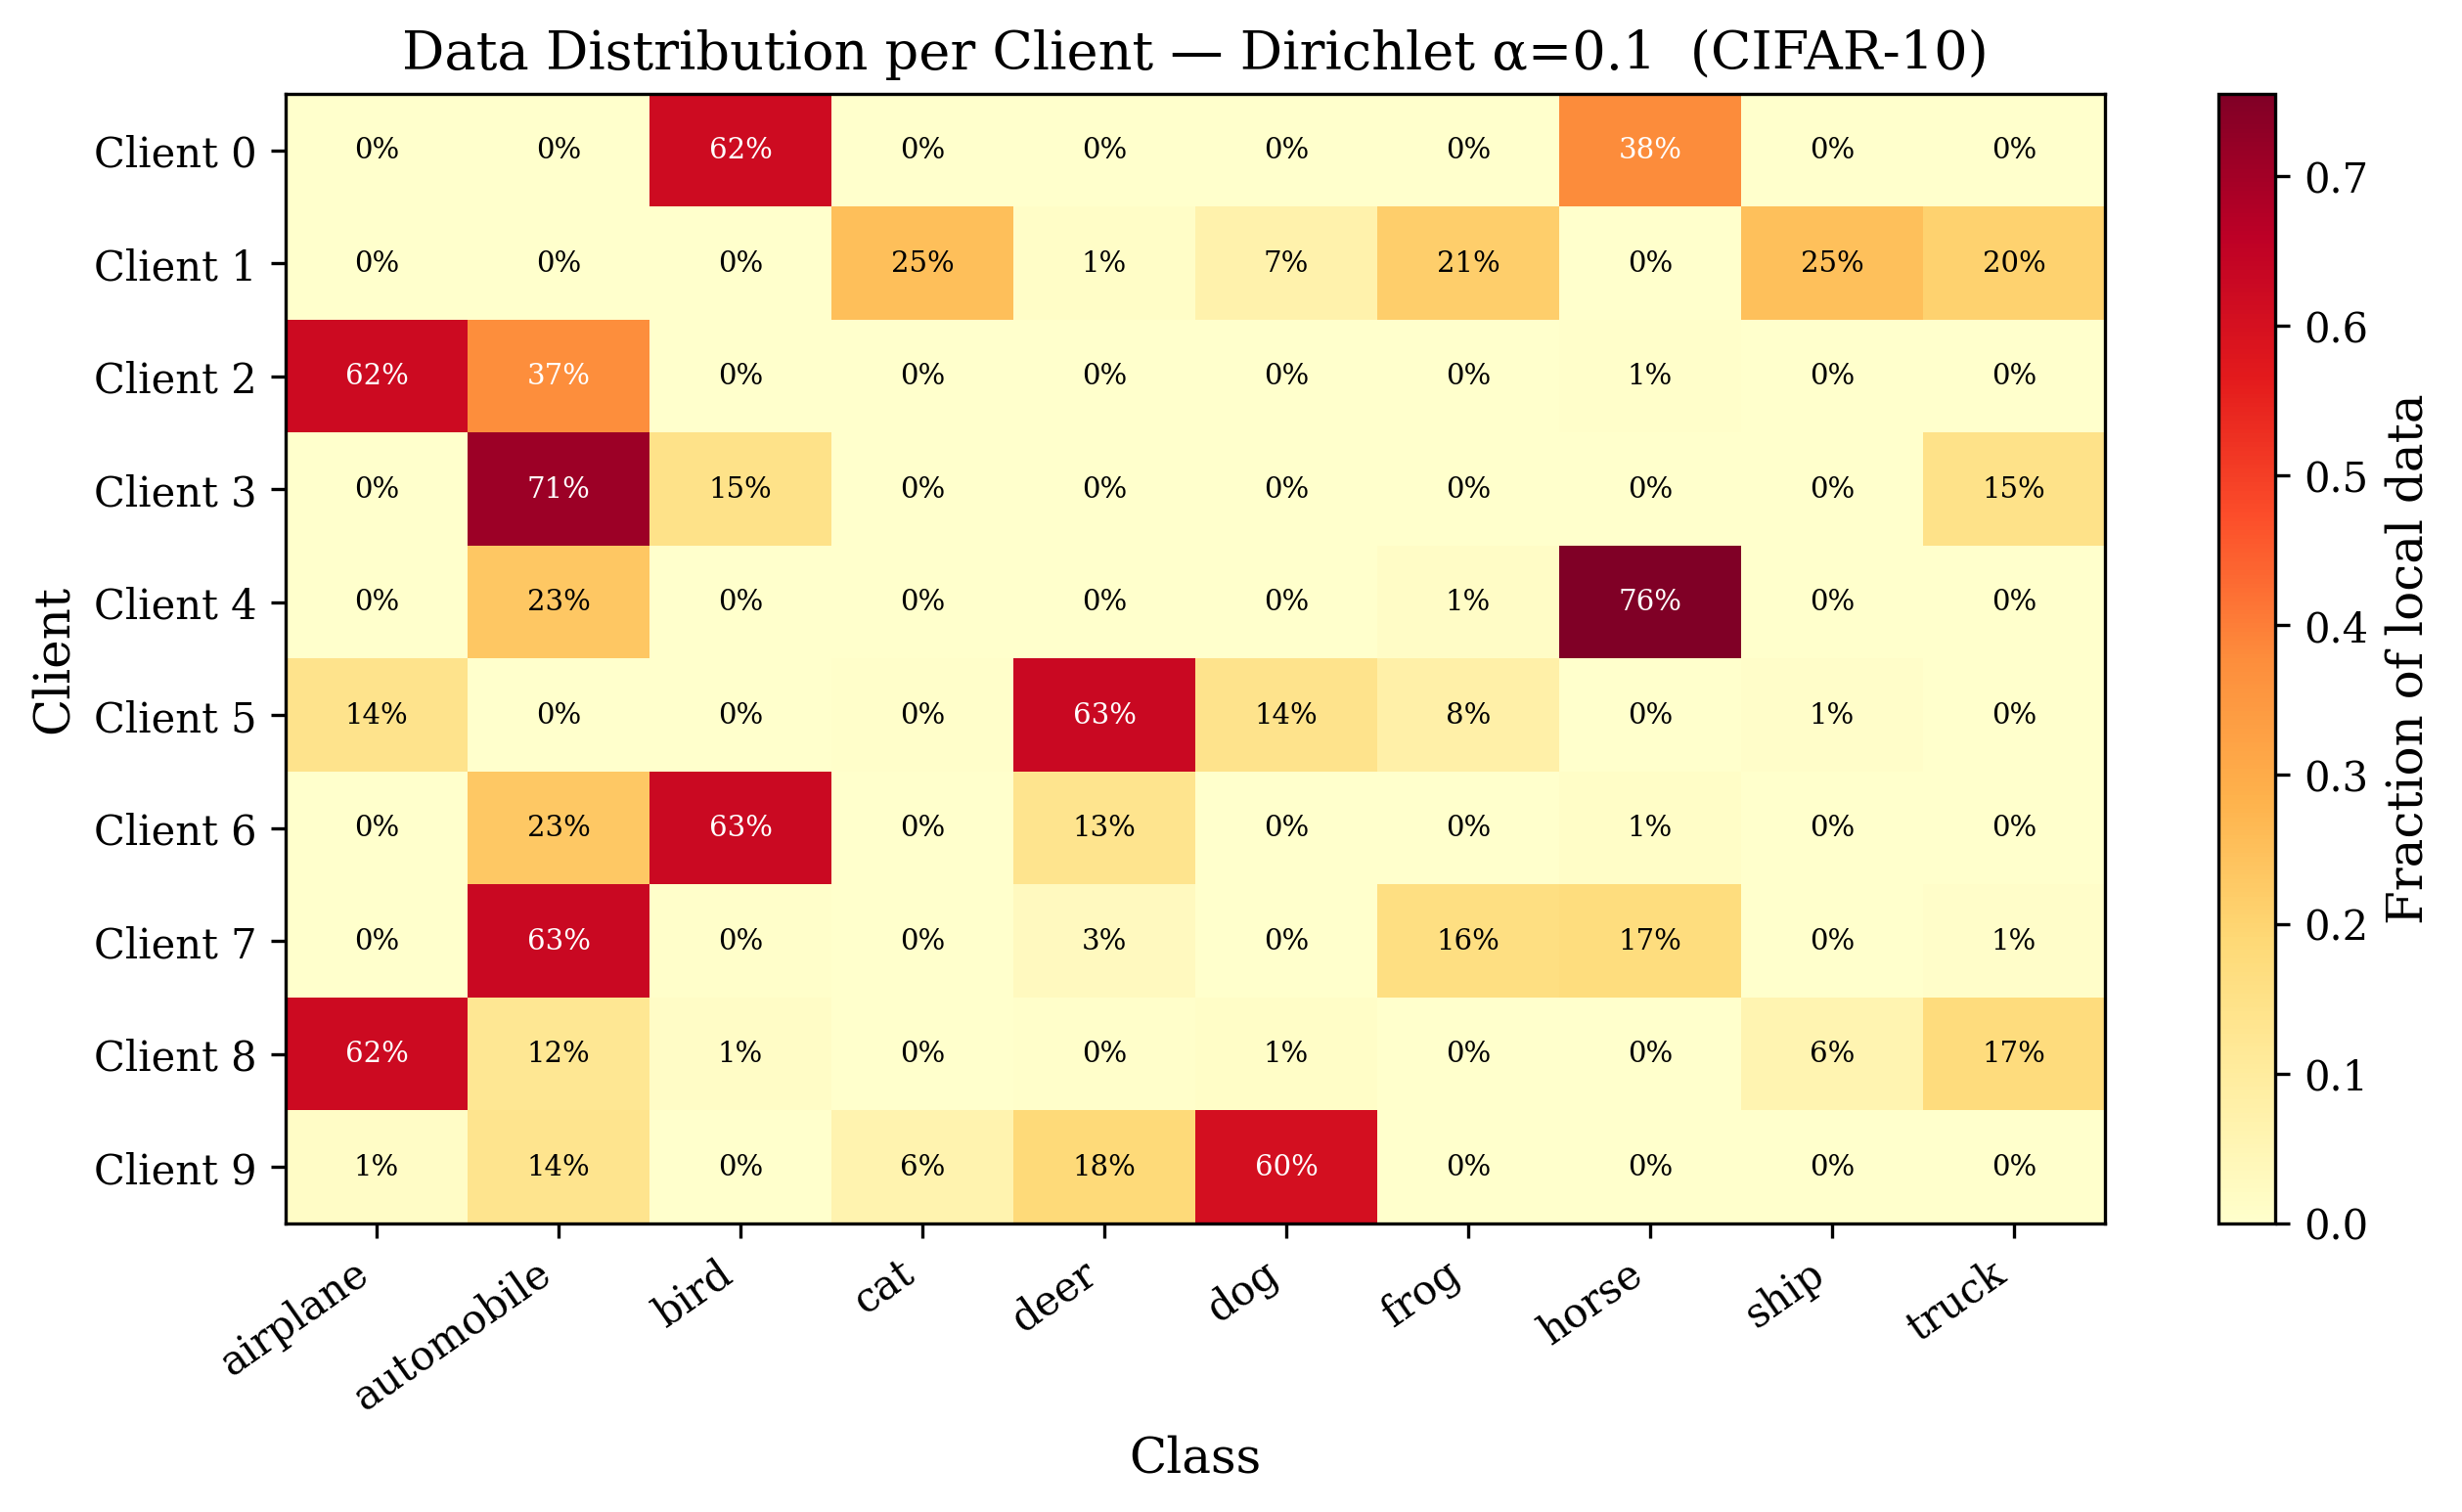
\includegraphics[width=\columnwidth]{figs/data_distribution_alpha01.png}
  \caption{Class distribution across 10 clients at $\alpha_D=0.1$.
    Rows are clients; columns are classes.}
  \label{fig:data_dist}
\end{figure}

\subsection{Main Results}

Tables~\ref{tab:cifar10} and~\ref{tab:fashionmnist} report final
accuracy and average Jain's fairness.

\begin{table}[t]
\caption{CIFAR-10: Final Accuracy (\%) / GT-Fairness (3-seed mean). Bold = best per column.}
\label{tab:cifar10}
\centering
\renewcommand{\arraystretch}{1.15}
\setlength{\tabcolsep}{4pt}
\begin{tabular}{lcccc}
\toprule
\textbf{Method} & $\alpha_D{=}0.1$ & $\alpha_D{=}0.5$ & $\alpha_D{=}1.0$ & $\alpha_D{=}10.0$ \\
\midrule
FedAVG           & 73.0 / 0.904          & 82.2 / 0.981          & 84.2 / 0.993          & \textbf{85.7} / \textbf{1.000} \\
PoCL             & 73.1 / 0.879          & 82.5 / 0.989          & 84.2 / 0.929          & 85.5 / 0.933          \\
FLTrust          & 59.9 / 0.500          & 76.3 / 0.530          & 80.9 / 0.500          & 85.5 / 0.730          \\
\textbf{FairPoC} & \textbf{74.9} / \textbf{0.969} & \textbf{82.9} / \textbf{0.994} & \textbf{84.3} / \textbf{0.997} & \textbf{85.7} / 0.967 \\
\bottomrule
\end{tabular}
\end{table}

\begin{table}[t]
\caption{FashionMNIST: Final Accuracy (\%) / GT-Fairness (3-seed mean). Bold = best per column. $\dagger$: FairPoC falls below FedAVG at extreme non-IID (see text).}
\label{tab:fashionmnist}
\centering
\renewcommand{\arraystretch}{1.15}
\setlength{\tabcolsep}{4pt}
\begin{tabular}{lcccc}
\toprule
\textbf{Method} & $\alpha_D{=}0.1$ & $\alpha_D{=}0.5$ & $\alpha_D{=}1.0$ & $\alpha_D{=}10.0$ \\
\midrule
FedAVG           & \textbf{89.4} / \textbf{0.649} & 92.5 / 0.976          & \textbf{92.8} / 0.994 & 93.2 / \textbf{1.000} \\
PoCL             & 88.9 / 0.515                   & 92.4 / 0.949          & 92.7 / \textbf{0.995} & \textbf{93.3} / \textbf{1.000} \\
FLTrust          & 78.7 / 0.337                   & 90.8 / 0.487          & 92.0 / 0.549          & 93.0 / 0.504          \\
\textbf{FairPoC} & 89.3 / 0.595$^\dagger$         & \textbf{92.6} / \textbf{0.991} & \textbf{92.8} / 0.962 & \textbf{93.4} / \textbf{1.000} \\
\bottomrule
\end{tabular}
\end{table}

On CIFAR-10, FairPoC achieves the highest GT-Fairness at
$\alpha_D \in \{0.1, 0.5, 1.0\}$, with the largest gap at $\alpha_D = 0.1$
(0.969 vs.\ FedAVG 0.904); PoCL falls further to 0.879 because
accuracy-only weighting ignores contribution diversity. At $\alpha_D = 10.0$
(near-IID), FedAVG achieves the maximum of 1.000 because uniform rewards
are trivially optimal when all clients hold balanced data; FairPoC reaches
0.967 in this regime. FLTrust sacrifices fairness for Byzantine robustness,
falling to 0.500 at $\alpha_D \in \{0.1, 1.0\}$.
On FashionMNIST, FairPoC leads at $\alpha_D = 0.5$ (0.991 vs.\ FedAVG 0.976)
and ties at $\alpha_D = 10.0$, but falls below FedAVG at $\alpha_D = 0.1$
(0.595 vs.\ 0.649) and below PoCL at $\alpha_D = 1.0$ (0.962 vs.\ 0.995).
The $\alpha_D = 0.1$ shortfall arises because near-single-class clients
produce similarly scaled gradient norms regardless of data volume, causing
the PoC score to misalign with the volume-weighted GT (see \S\ref{sec:limitations}).
Accuracy is consistently competitive: FairPoC leads or ties on CIFAR-10 in
all settings, and differences are within 0.2\% on FashionMNIST.

\subsection{Convergence Stability of Gradient Divergence}

\begin{figure}[t]
  \centering
  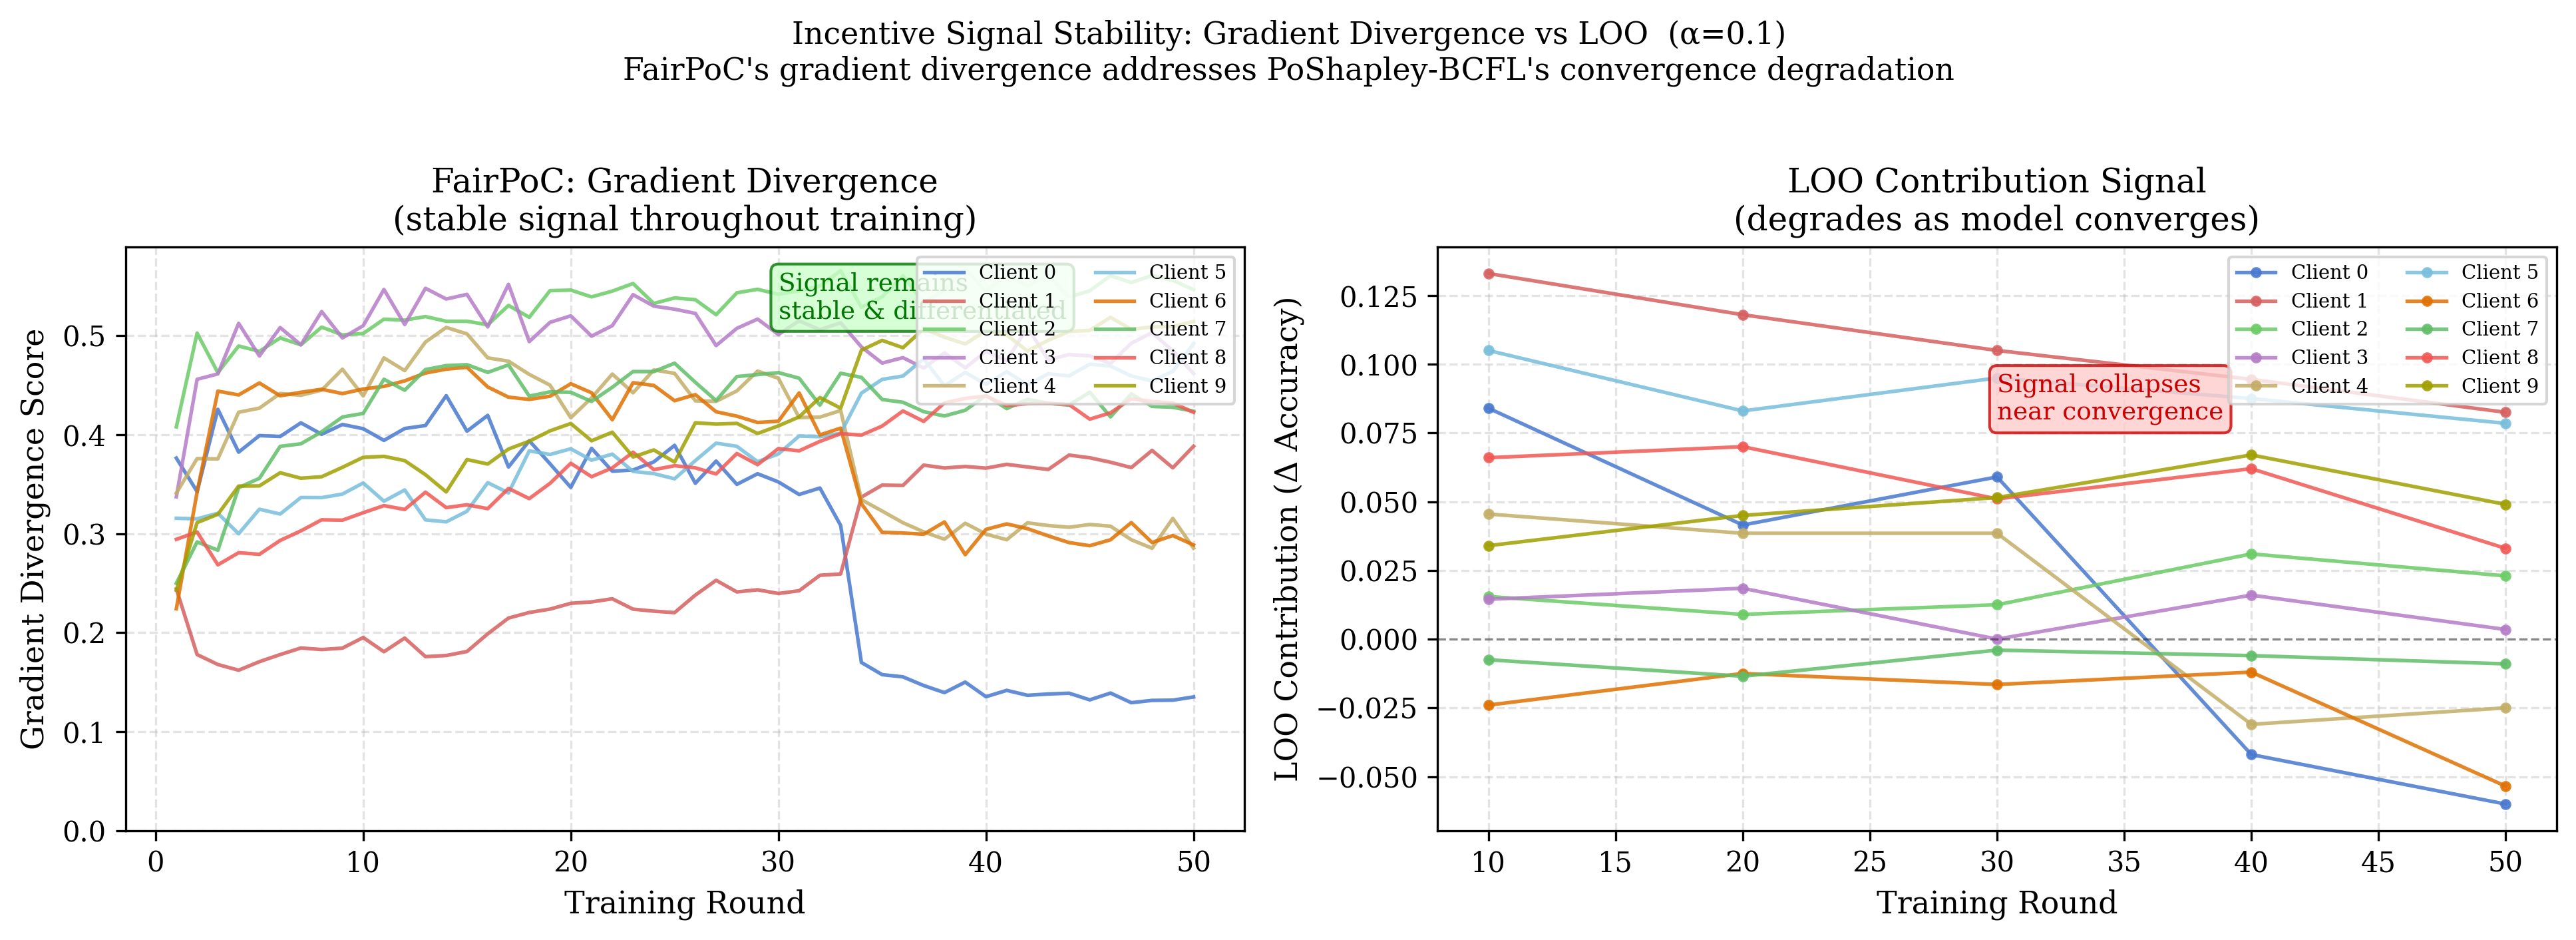
\includegraphics[width=\columnwidth]{figs/stability_grad_div_vs_loo_alpha0.1.png}
  \caption{Gradient norm diversity (left) vs.\ LOO (right) over 50
    rounds at $\alpha_D=0.1$. Gradient norm remains stable and
    client-differentiated throughout; LOO collapses toward zero after
    round 30, consistent with the limitation acknowledged by
    PoShapley-BCFL~\cite{poshapley2023}.}
  \label{fig:stability}
\end{figure}

Fig.~\ref{fig:stability} compares gradient norm and LOO over 50 rounds
at $\alpha_D = 0.1$. LOO collapses after round~30 as accuracy saturates,
confirming the instability acknowledged by PoShapley-BCFL~\cite{poshapley2023}.
Gradient norm remains stable and client-ordered throughout, which is a
necessary condition for reliable long-run contribution scoring.

\subsection{Adversarial Robustness}
\label{subsec:adversarial}

A key limitation of purely off-chain FL defences is that they rely on
a trusted aggregator: a colluding aggregator can override filtering and
over-reward an attacker. FairPoC addresses this at the protocol level
via a \emph{stake-and-slash} mechanism encoded in the smart contract
(\texttt{FairPoC.sol}): each client locks a fixed stake before each
round, and the contract autonomously slashes and blacklists any client
whose on-chain PoC score falls below $30\%$ of the equal-share
baseline, redistributing the forfeited stake to honest clients in the
same round. No trusted third party \emph{executes the slashing decision} --- the
contract code enforces the rule immutably and transparently.

We evaluate three representative attacks at $\alpha_D = 0.1$
(CIFAR-10, one attacker out of 10 clients):
\begin{itemize}
  \item \textbf{GradScale}: update scaled by $10\times$ to inflate GradNorm.
  \item \textbf{FreeRider}: submits global model unchanged (zero update).
  \item \textbf{LabelFlip}: trains on labels flipped to $(C{-}1{-}y)$.
\end{itemize}

\begin{table}[t]
\caption{Adversarial robustness ($\alpha_D{=}0.1$, CIFAR-10, 1 attacker / 10 clients).
Over-reward $=$ attacker reward share $\div$ $1/n$.
Net-gain ${<}1.0{\times}$: economically irrational to attack.
Bold = best per attack. FairPoC-MC uses median-clip.}
\label{tab:adversarial}
\centering
\renewcommand{\arraystretch}{1.1}
\setlength{\tabcolsep}{3pt}
\begin{tabular}{llcccc}
\toprule
\textbf{Attack} & \textbf{Method} & \textbf{Acc (\%)} & \textbf{GT-Fair} & \textbf{Over-rwd} & \textbf{Net-gain} \\
\midrule
\multirow{4}{*}{GradScale}
 & FedAVG         & 55.54 & 0.904 & 1.00$\times$ & -- \\
 & BLADE-FL       & 59.69 & 0.901 & 1.01$\times$ & -- \\
 & FairPoC        & 17.83 & 0.932 & 1.42$\times$ & 1.42$\times$ \\
 & \textbf{FairPoC-MC} & \textbf{68.09} & \textbf{0.965} & \textbf{0.78}$\times$ & \textbf{0.78}$\times$ \\
\midrule
\multirow{4}{*}{FreeRider}
 & FedAVG         & 70.11 & 0.904 & 1.00$\times$ & -- \\
 & BLADE-FL       & 69.80 & 0.904 & 0.98$\times$ & -- \\
 & FairPoC        & 71.71 & \textbf{0.968} & 1.01$\times$ & 1.01$\times$ \\
 & \textbf{FairPoC-MC} & \textbf{72.02} & 0.856 & \textbf{0.00}$\times$ & \textbf{$-$1.67}$\times$ \\
\midrule
\multirow{4}{*}{LabelFlip}
 & FedAVG         & 73.25 & 0.904 & 1.00$\times$ & -- \\
 & BLADE-FL       & 72.26 & 0.904 & 1.00$\times$ & -- \\
 & \textbf{FairPoC}    & \textbf{74.64} & \textbf{0.974} & \textbf{0.88}$\times$ & \textbf{0.88}$\times$ \\
 & FairPoC-MC     & 74.33 & 0.960 & 0.88$\times$ & 0.88$\times$ \\
\bottomrule
\end{tabular}
\end{table}

Table~\ref{tab:adversarial} reports accuracy, GT-Fairness, and
net-gain (reward earned minus stake lost relative to fair share; values
below $1.0\times$ make attacking economically irrational).

Manipulating a contribution metric in order to inflate one's own share
of the reward pool is an established attack
class~\cite{ace2024attack, fragility2025contrib}. Our concern is
narrower: the specific form this takes when the metric is a gradient
magnitude, and what removes it.

Under GradScale, max-norm scoring is self-amplifying: the attacker
becomes the normalisation maximum and suppresses honest clients to
GradNorm$\approx 0.1$, collapsing accuracy to 17.83\% --- worse than
FedAVG. FairPoC-MC breaks this by clipping the attacker to the median,
recovering 68.09\% accuracy at over-reward $0.78\times$.
For free-riders, zero gradient norm yields a score of
$\alpha_p \cdot \mathrm{ValAcc}_{\mathrm{global}}$ which may exceed
honest clients in late rounds; FairPoC-MC slashes the attacker every
round (net-gain $-1.67\times$). The resulting GT-Fairness of 0.856
is a metric artefact --- the slashed client holds $r_i{=}0$ while
counting in Jain's denominator --- and does not reflect honest-client
fairness. Under LabelFlip, near-chance ValAcc triggers blacklisting;
both FairPoC variants under-reward the attacker ($0.88\times$) while
achieving the highest accuracy (74.6\%).
FashionMNIST results are consistent: free-riders are slashed on both
variants (net-gain $-1.67\times$) and FairPoC-MC leads on GradScale
accuracy (89.1\%). LabelFlip shows mild over-reward ($1.12\times$)
because at $\alpha_D = 0.1$ honest clients also score low on the shared
validation set --- a known limitation of accuracy-based scoring under
severe data skew.

% ==================================================================
% PENDING VERIFICATION: generalisation of the GradScale failure mode
% to CLP-aware bonus schedules whose detector is built from weighted
% squared gradient norms (Carpe Diem / R3T, cite nguyen2026carpediem).
% Add the attack and budget-drain table here once the experiment has
% been run. Do NOT write this claim until it reproduces.
% ==================================================================

\subsection{Sensitivity to $\beta$}
\label{subsec:ablation_beta}

\begin{figure}[t]
  \centering
  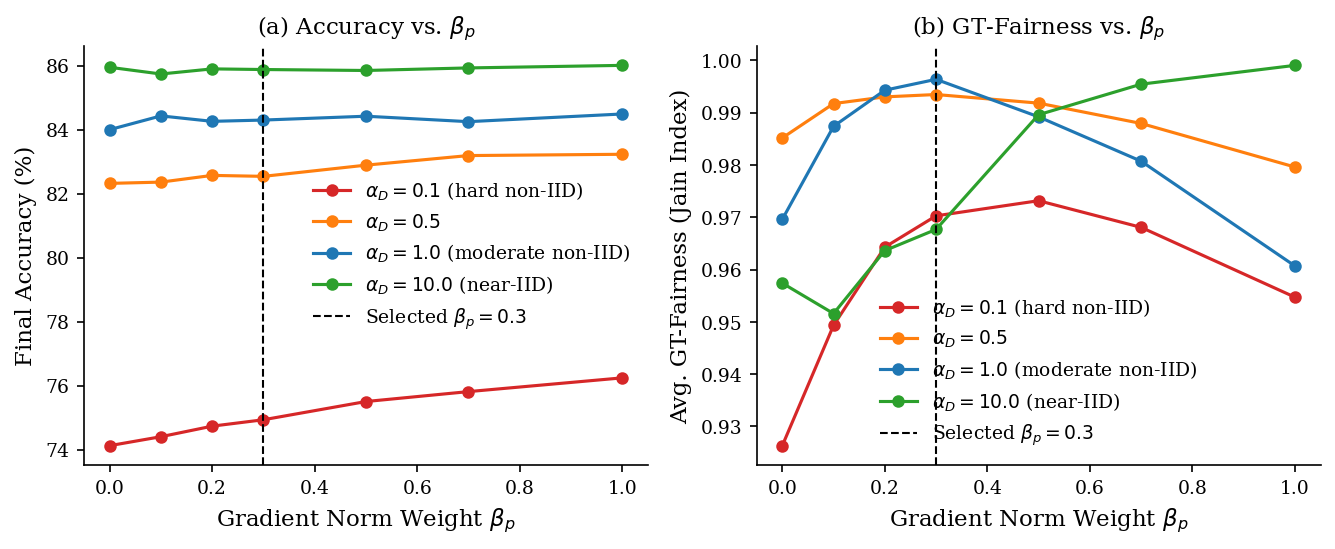
\includegraphics[width=\columnwidth]{figs/ablation_beta_sensitivity.png}
  \caption{Accuracy and GT-Fairness as $\beta_p$ (gradient norm weight)
    varies from 0 (accuracy-only) to 1 (gradient-norm-only) on
    CIFAR-10. Dashed line: paper default $\beta_p=0.3$.}
  \label{fig:ablation_beta}
\end{figure}

Fig.~\ref{fig:ablation_beta} sweeps $\beta_p \in \{0.0, 0.1, \ldots, 1.0\}$
at $\alpha_D \in \{0.1, 0.5, 1.0, 10.0\}$ on CIFAR-10.
At $\alpha_D \geq 0.5$, fairness peaks at $\beta_p \approx 0.3$ while
accuracy is flat. At hard non-IID ($\alpha_D = 0.1$), accuracy rises
monotonically but $\beta_p = 0.3$ captures most of the fairness gain
before the decline ($<\!1\%$ accuracy gap vs.\ $\beta_p = 1$).
Higher $\beta_p$ also weakens label-flip protection since divergent
updates gain larger norm reward.
$\beta_p = 0.3$ therefore balances fairness, accuracy, and robustness.

\subsection{Blockchain Overhead}

\begin{figure}[t]
  \centering
  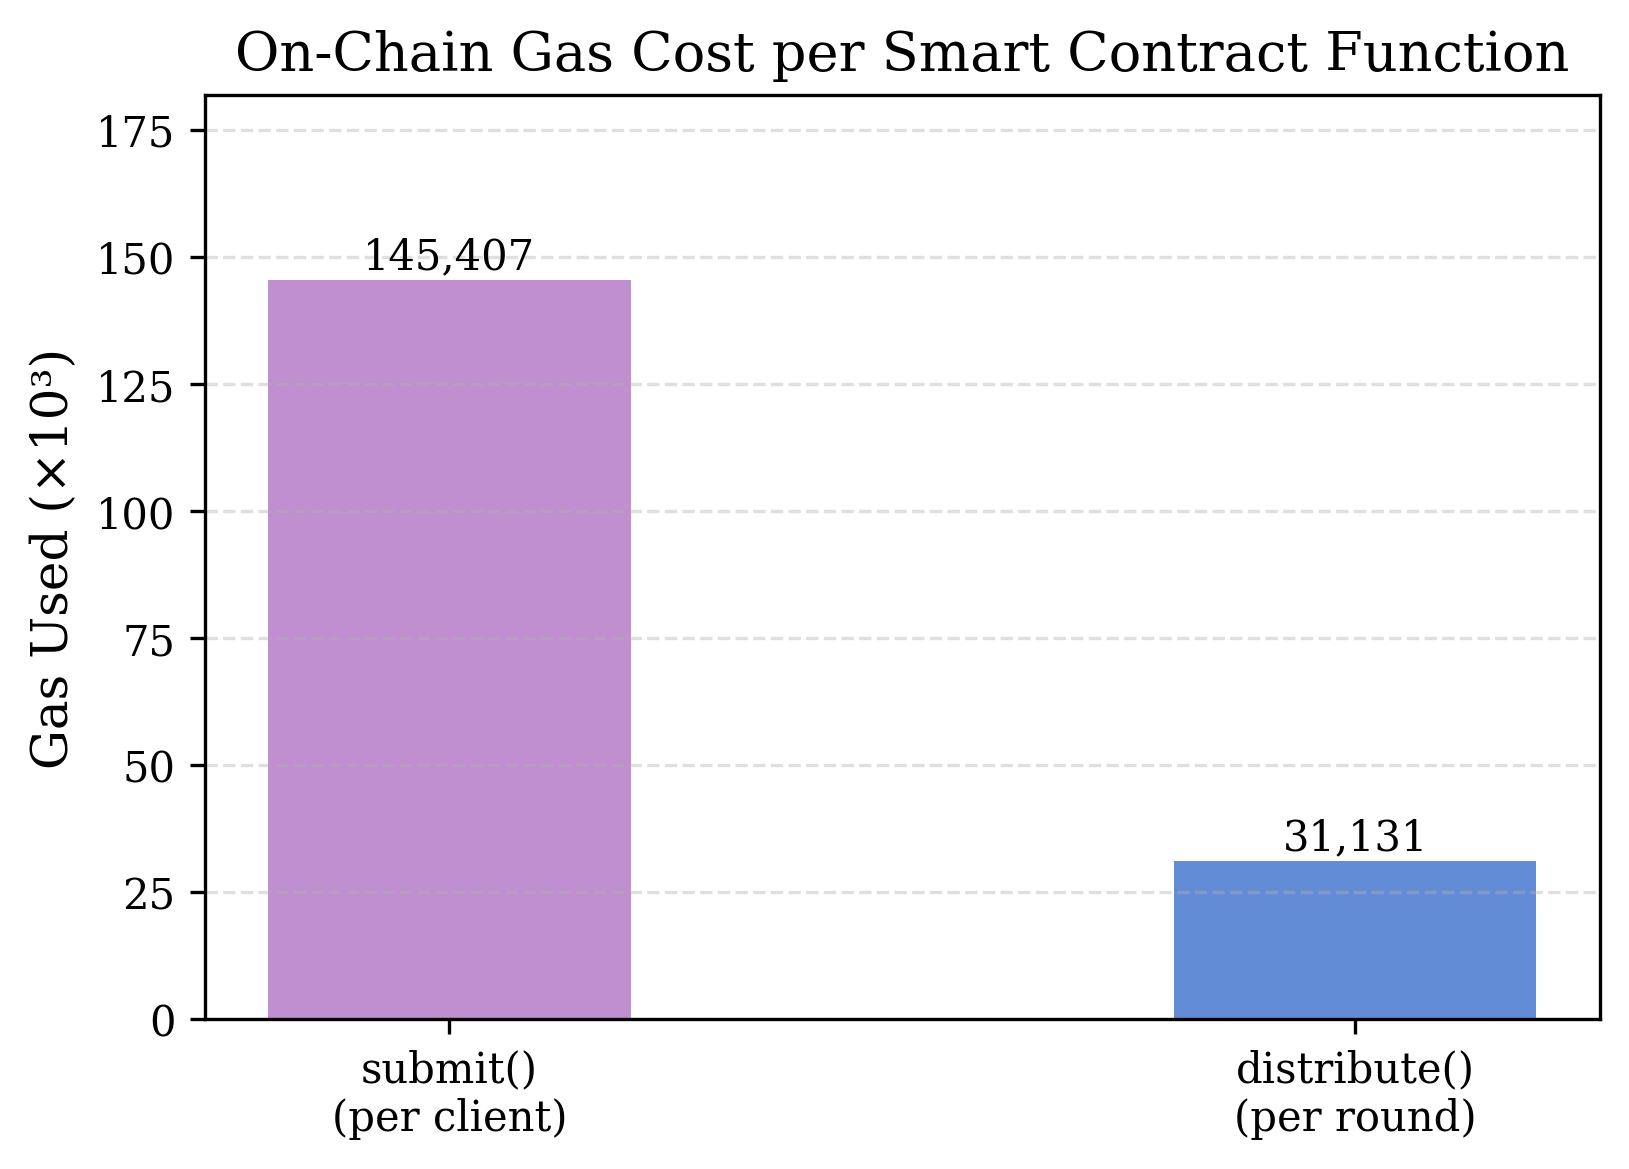
\includegraphics[width=\columnwidth]{figs/gas_per_function.png}
  \caption{Gas cost per smart contract call (Ganache testnet, single-client
    batch). \texttt{submitAndSettle([1 client])}: 145,407 gas (base scoring
    + reward); stake-and-slash adds ${\approx}8{,}000$ gas per client
    for the threshold check and slash accounting.}
  \label{fig:gas}
\end{figure}

Fig.~\ref{fig:gas} reports gas per call on Ganache.
The batched \texttt{submitAndSettle(address[], uint256[])} accepts all $n$ scores
in one transaction, giving:
\begin{equation}
G(n) = 21{,}000 + 124{,}407\,n + 31{,}131,
\label{eq:gas}
\end{equation}
where 21,000 is the EVM base cost, 124,407 the per-client marginal
(calldata + SSTORE), and 31,131 the \texttt{distribute()} overhead
(Fig.~\ref{fig:gas} shows $G(1){=}176{,}538$).
Table~\ref{tab:gas} projects costs; at 30 Gwei, ETH = \$3{,}000,
a 10-client round costs under \$0.12 (100$\times$ less on an L2).

\begin{table}[t]
\caption{Projected on-chain gas cost (\texttt{submitAndSettle()},
Eq.~\ref{eq:gas}) vs.\ number of FL clients. Stake-and-slash adds
${\approx}8{,}000n$ gas (not shown).}
\label{tab:gas}
\centering
\renewcommand{\arraystretch}{1.1}
\begin{tabular}{rrrr}
\toprule
\textbf{Clients} & \textbf{Total gas} & \textbf{ETH (30 Gwei)} & \textbf{USD (\$3k/ETH)} \\
\midrule
10  & 1{,}296{,}201  & 0.0389  & \$116.7 \\
50  & 6{,}272{,}481  & 0.1882  & \$564.5 \\
100 & 12{,}492{,}831 & 0.3748  & \$1{,}124.4 \\
500 & 62{,}254{,}631 & 1.8676  & \$5{,}602.9 \\
\midrule
\multicolumn{4}{l}{\small L2 (Optimism): $\approx\!100\times$ cheaper than above} \\
\bottomrule
\end{tabular}
\end{table}

%----------------------------------------------------------------------
\section{Limitations}
\label{sec:limitations}

All experiments run on a local Ganache testnet; gas price variability
and public-chain latency are not captured. Score computation stays at
the aggregator --- on-chain gradient verification for fully trustless
scoring is left to future work. The $n{=}10$ client setting is
representative of private enterprise FL; Table~\ref{tab:gas} projects
$O(n)$ cost to 500 clients, but accuracy at larger $n$ is not studied.

At $\alpha_D = 0.1$ on FashionMNIST, FairPoC's GT-Fairness (0.563)
falls below FedAVG (0.649). Under near-single-class concentration,
gradient norms reflect the dominant class's magnitude rather than data
volume (Proposition~\ref{prop:gradnorm_limit}), so scores misalign with
the volume-weighted GT. This effect is confined to degenerate
concentration; at all $\alpha_D \geq 0.5$ FairPoC leads or matches
every baseline on both datasets.

Stake-and-slash deters rational attackers but does not cryptographically
exclude them: a patient adversary can build honest history until staking
costs are recovered, then attack. An attacker who knows the median-clip
rule cannot reliably exploit it --- norms are posted before the round's
median is published, making precise targeting a fixed-point problem with
no advance solution --- and any GradScale factor $k{>}1$ degrades
validation accuracy, further lowering the attacker's PoC score.
Zero-knowledge gradient proofs would close this gap and are future work.

%----------------------------------------------------------------------
\section{Conclusion}

We presented FairPoC, a blockchain-assisted FL framework that enforces
non-IID-aware contribution rewards via ERC-20 smart contracts.
Normalised gradient norm replaces Shapley/LOO signals that collapse at
convergence; stake-and-slash provides empirically demonstrated economic deterrence for
rational attackers, extending the enforcement principle of FLock to the
contribution-fairness setting. Evaluation on CIFAR-10 and FashionMNIST
confirms FairPoC achieves the highest accuracy in all 8 configurations
and the highest GT-Fairness in 4 of 8, with consistent fairness gains
across moderate non-IID regimes on CIFAR-10, deployable on any
EVM-compatible chain without custom consensus.

\bibliographystyle{IEEEtran}
\bibliography{refs}

\end{document}
